\documentclass[11pt]{article}
\setlength{\parindent}{0pt}
\usepackage{graphicx}
\graphicspath{ {./} }
\setlength{\parskip}{1em}

\usepackage{fullpage}

\begin{document}

\title{ARM Final Report}
\author{J. Bae, A. Reynaldi, R. Rusly, P. Mazurina}

\maketitle

\section{Assembler}
\subsection{Assembler Structure}
\begin{figure}[h]
  \centering
  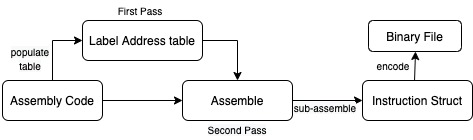
\includegraphics[width=0.7\linewidth]{assembler_structure.jpeg}
  \caption{High-level representation of the assembler.}
\end{figure}
Each box in the diagram represent a product of the function, except the ‘Assemble’ box which represents a process. The functions are the arrows pointing to the box.

The data flow followed a 2-pass approach, with each pass processing the assembly file line-by-line:
\begin{enumerate}
    \item \textbf{First pass:} we create a symbol table which maps string to integer. Through the lines, labels are collected and mapped to the memory location they represent, populating the symbol table. We keep track of the current address (memory locaiton) as we go through the lines. By the end of the first pass, address represents how many bytes are needed to store the instructions hence the output size.
    \item \textbf{Second pass:} For every instruction, we pass it into the assemble function which returns an unsigned integer. By the function, each non-label line is assembled into a 32-bit word and stored on the output array of type unsigned char.
\end{enumerate}
Given the array of bytes with the output after the second pass, we then write the output into the binary file.

\subsection{Symbol Table ADT}
For the assembler, we used an Abstract Data Type called symbol table. This table is implemented as a linked list ordered lexically according to the keys. There are 2 types of symbol table that we implemented and used:
\begin{itemize}
    \item \textbf{table:} Symbol table with key of type string and value of type integer. We use this to map the label (\verb|string|) to their memory address (\verb|unsigned integer|).
    \item \textbf{ftable:} Symbol table with key of type string and value of type function pointer. We use this table to map an instruction’s mnemonic opcode (\verb|string|) to an assembly function of the respective instruction type (\verb|void *|)
\end{itemize}

\subsection{Assemble function}
The assembly process for each line follows these steps:
\begin{enumerate}
    \item Create function table (\verb|ftable|) which maps instructions’ mnemonic opcode to function pointer.
    \item Tokenize the line into opcode and operands with token function which returns the number of tokens in a line.
    \item Get the function pointer to the instruction-specific assemble function from the function table using the tokenized mnemonic opcode as a key.
    \item Call the retrieved function by passing the tokens, number of tokens, and details for the output into the function pointer. The function returns the instruction encoded as \verb|unsigned int|.
    \item Convert the encoded instruction from \verb|unsigned int| to \verb|unsigned char[4]| in little-endian mode.
\end{enumerate}

The assemble function then returns new size of output (used to write output into the binary file) since the assembly process of single data transfer instructions may modify the size of output while appending the additional data at the end of the file.

The instruction specific assemble functions must all have the same signature, so they are encapsulated in container functions that we generated using macros. Many instructions also share the same implementation, so this code style allows the implementation of only one (or two) function(s) for each category of instruction, instead of having to implement one assemble function for each instruction type. The instruction-specific assemble functions then parse the tokens to construct the encoded instruction.

\section{Extension - ARMShake}

In 2001, Karl Hasselström and Jon Åslund designed the Shakespeare Programming Language (SPL), a programming language that resembled Shakespeare’s plays. This language turned programming into a matter of poetry. We aim to do the same for ARM assembly with our project extension: a compiler for a subset of SPL, producing assembly code compatible with part II of the project (and, by transitivity, part I as well).

An SPL program is a play where variables appear in the form of characters. Dialogue lines translate into data processing assembly commands, and act \& scene declarations translate into labels. For more details on the language, please see the Appendix where we have included a description of the language.

\subsection{Example}
\begin{verbatim}
The Shakespearian one plus one.

Macbeth, a young king aiming to catch them all and become number one.
Banquo, Macbeth’s rival who wants to be the very best, like no one ever was.
Duncan, who aims to unite the two rivals for eternal glory.

Act I: A banquet for the lords.
Scene I: The achievements of young rivals.

[Enter Macbeth, Banquo]

Macbeth:
Thou art as glorious as a lord!

Banquo:
You genius!

[The two best friends playfully wrestle as they disappear into the banquet hall]
[Exeunt]

Scene II: The reunions.

[Enter Macbeth, Duncan]

Macbeth:
Thou art as awesome as the sum of Banquo and thyself!

[Exit Macbeth]
[Enter Banquo]

Banquo:
You are as glorious as the sum of Macbeth and yourself!

[Exeunt]
\end{verbatim}
The above program translates into the following assembly:
\begin{verbatim}
a1s1:
ldr r1, =1
ldr r0, =1
a1s2:
add r2, r1, r2
add r2, r0, r2
\end{verbatim}

\subsection{Program Structure}

At first, we populate a symbol table using the Dramatis Personae. The Dramatis Personae is a declaration of characters involved in the play, and within the context of an SPL program they can be treated as variables. We have chosen to interpret each character as a separate register, so any play can only have 13 characters at most.

The program is then split into lines delimited by punctuation marks. There are 2 kinds of lines: the first kind consists of lines that do not translate to machine code but do provide context for translating the next lines. These include stage directions, dialogue specifiers (i.e. which character is talking right now) and act declaration. The second type are lines that do translate into actual assembly, which include scene declarations and dialogue lines.

Each line is further parsed into tokens, and the parsing of each line can be modelled with a finite state machine where state transitions are determined by the current token. Ideally, each state would be represented by a single function which calls the next appropriate function depending on the current token. However, some states are terminal, in the sense that once we have entered that state we definitely know how it will end (assuming a syntactically correct program). This allows us to group multiple states in one function, thereby minimizing the number of functions.

\subsection{Challenges}

Implementing the tokenizer was challenging because we had to tokenize twice: once to split into lines, and another time to split the line into words. The line tokenizer required that we kept the delimiter (the punctuation) as part of the line. The word tokenizer required certain delimiters (i.e. the punctuation) to be parsed as a separate token. In the end, we decided to implement a parser from scratch that reads the string character by character, which gave us fine-tuned control over what to do with delimiters.

\subsection{Testing}

For testing we wrote a number of SPL files and compiled them by hand into assembly. We then built a testing framework that verifies the output of the compiler matches the assembly file we wrote manually. Due to time constraints, we decided that unit testing the extension was not in our best interest, although the extension would have benefitted quite greatly from it. We feel our testing strategy was rather rudimentary, but nevertheless it allowed us to discover tokenization problems in our code that would not have shown itself.

\section{Reflection}
\subsection{Group Reflection}
We had quite a rough start because of the pandemic as well as different time zones. The biggest issues were coordinating and communicating our code, as some of us were initially afraid to make mistakes on gitlab, as well as ask each other for clarification. In the beginning, we did not discuss the whole project but discussed only part I, which left the remaining tasks uncertain as to their division. This meant that some members couldn’t really get started on part II until we discussed it again, and the group only had a meeting 1 - 2 times a week. For future projects, we think we will have to meet more often, and encourage each other to ask questions so that everyone is on the same page.

\subsection{Individual Reflection}
\subsubsection{Alexander Reynaldi}
Initially, I expected that everyone would be just as enthusiastic as me to start the group project. Especially with the pandemic, I was eager to start a fun project. However as the project started it became clear that this is not the case. In particular, I expected some of my teammates to immediately start working, which I understand now is not a realistic expectation given that I don't know much about their daily lives.

I feel like I am somewhat of a pedant: it has always annoyed me to see code written in a different way from what I expect. I thought this would help in keeping the project's code style consistent, but this group project has exposed me to different people's programming styles, and multiple times I've had to face the reality that my teammate's implementation is simply better than what I had conjured in my head. In fact, I've come to enjoy talking and finding out about their implementations and working together to fix bugs. I think this group project has taught me an important lesson in perspective, which I will keep in mind for future projects.
\subsubsection{Junhyuk Bae}
Having been responsible for the multiply and single data transfer in part 1, I have found that without proper communication (mostly due to the fact that this project is remote), it is very difficult to convey what the code does. I have found that I spent far more time trying to understand what my peers have written than writing my own code to contribute. This caused me to fall behind very often. Sometimes, when my knowledge of the code was inadequate, my code tended to be very unpolished, and my teammates would have to add onto my code. In the future, I would try to create more group sessions where we can go over the project as necessary.
\subsubsection{Rania Rusly}
In the process of working on the C project, I realized that enhanced communication is the most important given the current situation of working remotely and being in the different time zones. It was hard to work on the code together as we have limited group meetings due to different availibilities. As there is limitation in being able to meet directly face-to-face, it was also difficult to ensure that everybody is in the same page while having to progress quickly with the project. Having had previous experience in working for projects on gitlab, I spent a significant amout of time in combining, covering, and reviewing the work of my peers. For following projects, I would like to create much more frequent group meetings since it is also the key to unlock each member’s ability to contribute to the project.
\subsubsection{Polina Mazurina}
Sometimes due to lack of clarity in task division our goals overlapped, and different group members ended up doing the same task. More frequent meetings would’ve solved this problem.  Sometimes it was also hard to figure out how did the code of other team members work, and this resulted in various inconveniences, which included adding code snippets and variables to the places they didn’t belong to or mistaking over the use of implemented techniques. However, our decision to use branches on GitLab turned out to be a great idea, as it helped with eliminating mistakes and non-compiling parts, as well as sharing ideas and commenting on each other’s’ code. Nest time, the project like this will require much more clarity and meetings. 
\newpage
\section{Appendix I - The anatomy of SPL code}
SPL lines of code are delimited with punctuation marks, particularly periods and commas. A period or exclamation mark is generally used to delimit lines of code, with the exception of stage directions which use square brackets instead.

\subsection{Title}
All text until the first period/exclamation mark in the program is the title. This title is purely for cosmetic purposes.

Format: \verb|<title>|

Example: \verb|A Midsummer Night’s Program.|

\subsection{Dramatis Personae}
Characters are variables in the program, and they must be declared immediately after the title. Furthermore, characters must be Shakespeare characters.

Format: \verb|<Character Name>, <description>.|

\subsubsection{Example}
\begin{verbatim}
Romeo, a young man with the face of a Disney prince.
Juliet, a self-aware Artificial Intelligence.
Macbeth, the tragic king of McDonalds.
Hamlet, a pig.
\end{verbatim}

\subsection{Acts \& Scenes}
Acts and Scenes act as labels in the program (for goto statements). Every scene below an act belongs to that act, so each label is uniquely identifiable by the act and scene number. Of course, numbers are in Roman numerals. Each scene is a label to the next character line after that scene.

\subsubsection{Formats}
\begin{verbatim}
Act <act number>: <act title>.
Scene <scene number>: <scene title>.
\end{verbatim}

\subsubsection{Example}
\begin{verbatim}
Act I: The reckoning of power.
Scene I: A beautiful day at the park.
...
<some dialogue & stage directions...>
...
Scene II: <scene title>.
\end{verbatim}

\subsection{Stage Directions}

Each character/variable is either on or off the stage. Characters must be on the stage to speak their lines. The stage is emptied every time a new act or scene is entered. The stage can contain arbitrarily many characters, but having characters perform their lines when there are more than 2 characters on stage will cause a compile error (see “character lines” for an explanation).

\subsubsection{Formats}

Putting characters on stage:

\verb|[Enter <comma-separated list of characters>]|

Taking a character off stage:

\verb|[Exit <Exactly one character>]|

Taking multiple characters off stage:

\verb|[Exeunt <comma-separated list of characters>]|

Taking all characters off stage:

\verb|[Exeunt]|

Describing other actions (ignored by compiler, basically comment line):

\verb|[<Description of character actions>]|

\subsection{Character Lines}

A character line performs operations on the other character on the stage. If there are more than 2 characters on the stage when a line is spoken, a compile error will happen. This is because it becomes ambiguous who the target is. A character line must correspond to a single assembly operation. We can specify multiple lines spoken by a character at once, delimited by a period or exclamation mark.

\subsubsection{Format}
\verb|<Character name>: <line 1>. <line 2>! … <line n>.|

Example:
\begin{verbatim}
Hamlet: You lying stupid fatherless big smelly half-witted coward!
You are as stupid as the difference between a handsome rich brave
hero and thyself! You are as brave as the sum of your fat little
stuffed misused dusty old rotten codpiece and a beautiful fair warm
peaceful sunny day. You are as healthy as the difference between the
sweetest reddest rose and my father! You are as cowardly as the sum
of yourself and the difference between a big mighty proud kingdom and a horse.
\end{verbatim}

\subsection{Character Lines: Assignment of Value}

One type of character line assigns a value to the target. This is done either by calling the other character some noun preceded with a set of adjectives (constant value) or using a simile to describe some adjective of the target (arithmetic/logic operator). For more information, see the respective sections.

\subsubsection{Formats}

\verb|You <constant>!|

\verb|You are as <adjective> as <operator>.|

“you” may be replaced with “thou” and “are” may be replaced with “art”.

\subsubsection{Examples}

You big fat donkey.

Thou art as beautiful as the difference between Hamlet and a dumb fool.

\subsection{Constant Values}

Constant values are specified using a noun, possibly preceded by a whitespace separated list of adjectives. A noun has a value of either 1 or –1. Each adjective multiplies the constant value by 2.

Format:
\verb|<adj1> <adj2>  … <adjn>  <noun>|

\subsubsection{Example}
\begin{verbatim}
Thou
  |- good demon => ldr rd, =-2
  |- strange horrible person => ldr rd, =4
  |- massive massive large big apple => ldr rd, =16
\end{verbatim}

\subsection{Operators}

Operators can be specified with keyword(s) denoting the operation, followed by a connective word. The two inputs are then specified, separated by an “and”. We can also use the name of any other character in the play as an operator, which evaluates to that character’s current value. Ideally, we want to be able to nest operators, but this will require more than one assembly instruction per line. Therefore, inputs can only be constants or a character. In all cases, the destination register is the target of the line: the character who is currently not talking.

\subsubsection{Formats}
\begin{verbatim}
<operator keyword> of <character> and <const/character>
\end{verbatim}
\begin{verbatim}
<Operator keyword>
  |-"the sum" ==> add
  |-"the product" ==> mul (no constants allowed, as per the mul instruction)
  |-"the conjunction" ==> and
  |-"the disjunction" ==> orr
\end{verbatim}
\begin{verbatim}
the difference between <character> and <const/character> ==> sub
\end{verbatim}
\begin{verbatim}
<const> = a <constant>
\end{verbatim}
Note: the quantifier “a” can be replaced with any word, allowing the use of ”an”, ”my”, “thy”, “thine” or possessives, for example "Mozart's".

\begin{verbatim}
<character> = <character’s name>
\end{verbatim}
“thyself”, “you” and “yourself” works as a synonym for the current target’s name.
Just specifying the character name (without an operator) works too, in which case it’s a \verb|mov| from that character to the target.
\begin{verbatim}
<const>
\end{verbatim}
Specifying a single constant is the same as an ldr with a constant value.

\subsubsection{Example}
\begin{verbatim}
You are as dumb as
  |-the conjunction of Hamlet and a heavy rock. => and rd, r3, #2
  |-the difference between Juliet and a naked man. => sub rd, r1, #2
  |-Macbeth! => mov rd, r2
  |-a stupid blind cow => ldr rd, =4
\end{verbatim}
\end{document}
